\documentclass[bibliography=numbered,listof=numbered,11pt,a4paper,,oneside,openany,ngerman,plainfootsepline,plainheadsepline]{scrbook}
% Change "article" to "report" to get rid of page number on title page
\usepackage{amsmath,amsfonts,amsthm,amssymb}
\usepackage{setspace}
\usepackage{Tabbing}
\usepackage{lastpage}
\usepackage{cite}
\usepackage{tocbasic}
\usepackage[automark,						%Automatische Kopfzeile
						%headtopline,				%Linie über dem Seitenkopf
						%plainheadtopline,	%Plain, Linie über dem Seitenkopf
						headsepline,				%Linie zwischen Kopf und Textkörper
						%plainheadsepline,	%Plain, Linie zwischen Kopf und Textkörper
						footsepline,				%Linie zwischen Textkörper und Fuß
						plainfootsepline,   %Plain, Linie zwischen Textkörper und Fuß
						%footbotline,				%Linie unter dem Fuß
						%plainfootbotline   %Plain, Linie unter dem Fuß
						]{scrpage2}
\usepackage{graphicx,wrapfig}
%\usepackage[ansinew]{inputenc}
\usepackage{lmodern}
\usepackage{scrpage2}
\usepackage[utf8]{inputenc}
\usepackage[ngerman]{babel}
\usepackage[german=quotes]{csquotes}

\usepackage{listings}
\usepackage{color}
\definecolor{javared}{rgb}{0.6,0,0} % for strings
\definecolor{javagreen}{rgb}{0.25,0.5,0.35} % comments
\definecolor{javapurple}{rgb}{0.5,0,0.35} % keywords
\definecolor{javadocblue}{rgb}{0.25,0.35,0.75} % javadoc

%\usepackage{url}
\usepackage{hyperref}
	\hypersetup{hidelinks=true}
\usepackage{fouriernc}
%\usepackage[scaled]{helvet}
\renewcommand*\familydefault{\sfdefault} %% Only if the base font of the document is to be sans serif
%\usepackage[T1]{fontenc}
% In case you need to adjust margins:
\topmargin=-0.45in      %
\evensidemargin=0in     %
\oddsidemargin=0in      %
\textwidth=6.5in        %
\textheight=9.0in       %
\headsep=0.25in         %
\setcounter{secnumdepth}{3}
\setcounter{tocdepth}{3}

% Homework Specific Information
\newcommand{\hmwkAuthorName}{Ramon Schilling}
\newcommand{\hmwkTitle}{Seminar Hibernate}
\newcommand{\hmwkClass}{Seminar Hibernate\\ZHAW - Zürcher Hochschule für Angewandte Wissenschaften}
\newcommand{\hmwkVersion}{Version 1.0}

\clearscrplain		
%Alte Plain-Formatierung entfernen
\clearscrheadfoot
\cehead{\headmark}    % Chapter auf geraden Seiten (links) in Kopfzeile
\cohead{\headmark}
\rehead{
\includegraphics[width=50pt]{graphics/logo_zhaw_soe.png}}    % Logo auf geraden Seiten (rechts) in Kopfzeile
\rohead{
\includegraphics[width=50pt]{graphics/logo_zhaw_soe.png}}    % Logo auf ungeraden Seiten (links) in Kopfzeile
\lehead{\hmwkTitle}    % Section auf geraden Seiten (rechts) in Kopfzeile
\lohead{\hmwkTitle} 

\lefoot{\hmwkAuthorName}    % Chapter auf geraden Seiten (links) in Kopfzeile
\lofoot{\hmwkAuthorName}
\cefoot{\hmwkVersion}
\cofoot{\hmwkVersion}
\rofoot{Seite\ \thepage\ von\ \pageref{LastPage}}    % Chaper auf geraden Seiten (links) in Kopfzeile
\refoot{Seite\ \thepage\ von\ \pageref{LastPage}}
\setheadsepline{0.4pt}
\setfootsepline{0.4pt}

\pagestyle{scrheadings}
\automark[chapter]{chapter}
 % Seitenstil aktivieren
\renewcommand{\chapterpagestyle}{scrheadings}
% This is used to trace down (pin point) problems
% in latexing a document:
%\tracingall


%%%%%%%%%%%%%%%%%%%%%%%%%%%%%%%%%%%%%%%%%%%%%%%%%%%%%%%%%%%%%
% Make title
\title{\vspace{2in}\textmd{\textbf{\ \hmwkTitle}}\\\normalsize\vspace{0.1in}\large{\hmwkClass}\\\vspace{0.1in}\large{\textit{}}\vspace{3in}}

%\author{\textbf{\hmwkAuthorName}}
\author{\textbf{Ramon Schilling}\\schilram@students.zhaw.ch}
%%%%%%%%%%%%%%%%%%%%%%%%%%%%%%%%%%%%%%%%%%%%%%%%%%%%%%%%%%%%%
\begin{document}
\begin{spacing}{1.1}
\maketitle
\newpage
% Uncomment the \tableofcontents and \newpage lines to get a Contents page
% Uncomment the \setcounter line as well if you do NOT want subsections
%       listed in Contents
%\setcounter{tocdepth}{1}
%\tableofcontents
%\newpage
% When problems are long, it may be desirable to put a \newpage or a
% \clearpage before each homeworkProblem environment
\pagenumbering{arabic}  %1, 2, 3, 4, ...
\setcounter{page}{1}
\clearpage
\begin{normalsize}
\setcounter{tocdepth}{2}
\tableofcontents
\end{normalsize}

\chapter{Einleitung}
\label{chap:Einleitung}
Dieses Dokument wurde für das Seminar \enquote{SW Entwicklung mit Hibernate} geschrieben.

\section{Aufgabenstellung}
\begin{itemize}
	\item Einarbeitung in das Thema ORM mit Hibernate \cite{Hibernate}.
	\item Erestellung einer kleinen Anwendung mit Gui welche das Hibernate-Framework nutzt.
	\item Dokumentation welche die Architektur sowie die einzelnene Komponenten erklärt.
\end{itemize}


\section{Deliveries}
\begin{itemize}
	\item Source Code und lauffähiger Maschinencode.
	\item Dokumentation
\end{itemize}

\section{Zielsetzung}
Das Ziel der Seminararbeit ist es, das O/R-Mapping Paradigma am Beispiel des Hibernate Frameworks zu verstehen und eine Anwendung unter Verwendung dieses Frameworks zu implementieren.

\section{Motivation}
Da ich seit Oktober letzten Jahres als Java Entwickler arbeite, war für mich klar, dass ich ein Seminar wählen wollte mit welchem ich meine Entwicklungskenntnisse vertiefen und neue Erfahrungen sammeln kann. Da das Thema ORM bei der Entwicklung von Software sehr wichtig ist, da die meisten Applikationen irgendwie mit einer Datenbank arbeiten war die Wahl schnell gefallen. Wir arbeiten in der Firma auch mit Hibernate und setzen auch das Framework Spring \cite{Spring} ein. Da ich aber noch kein Projekt von Grund auf mitaufgebaut habe, wollte ich diese Arbeit als Chance nutzen nicht nur Hibernate genauer kennezulernen sonder auch Spring, bzw. Teile davon. Im Speziellen wollte ich Spring MVC und Spring Data genauer anschauen.

Zur Umsetzung der Anforderungen möchte ich eine Anwendung entwicklen in welcher Rezepte verwaltet werden können. Als Besonderheit soll es möglich sein nach Rezepten zu Suchen in dem man die vorhandenen Zutaten angibt. 
\chapter{Projektmanagement}
\label{sec:Projektmanagement}

\section{Projektplanung}
\begin{tabbing}
20. März 2013	\= -	\= Kick Off Meeting	\\
27. März 2013	\> -	\> Einreichen der Aufgabe \\
12. Juni 2013	\> -	\> Abgabe Schriftliche Arbeit und Anwendung	\\
19. Juni 2013	\> -	\> Präsentation	\\
\end{tabbing}


\section{Aufwand}
Der Aufwand für die Seminararbeit sollte 50 h betragen. \\

\begin{tabular}{|l|c|c|}
\hline 
\textbf{Beschreibung} & \textbf{Soll}& \textbf{Ist} \\ 
\hline 
Einarbeitung in Hibernate & 4 h & 2 h \\ 
\hline 
Einarbeitung in Spring & 4 h & 2 h \\ 
\hline 
Einrichten der Entwicklungsumgegbung inkl. Hibernate Test & 4 h & 8 h \\ 
\hline 
Programmieren der Anwendung & 28 h & 32 h \\ 
\hline
Dokumentation & 8 h & 8 h \\ 
\hline 
\textbf{Total} & \textbf{48 h} & \textbf{52 h} \\
\hline
\end{tabular}
\\\\
Die Aufwandschätzung fiel mir relativ schwer, was sich auch darin zeigt, dass die Soll und Ist Zeiten nicht übereinstimmen. Ich habe für die theoretische Einarbeitung in Hibernate und Spring weniger Zeit aufwendete als geplant um schneller mit der Umsetzung zu beginnen. Bis ich dann aber alles soweit konfiguriert hatte, dass das Object-Relation-Mapping funktionierte hatte ich viel mehr Zeit gebraucht als geplant. Beim Programmieren habe ich ebenfalls z.T. sehr viel Zeit gebraucht um Fehler zu finden welche ich mit etwas mehr Erfahrung wohl gar nicht erst gemacht hätte.

\section{Hilfsmittel}

\subsection{Versionskontrolle}
Um eine Versionskontrolle zu haben, habe ich in Github \cite{Github} ein Repository erstellt und sämtliche für das Projekt nötigen Dateien dort eingecheckt.

\subsection{Dokumentation}
Die Dokumentation habe ich mit \LaTeX{} erstellt. Als Editor habe ich TeXnicCenter \cite{TeXnicCenter} genutzt.

\subsection{Programmierung}
Als Entwicklungsumgebung für die Java Programmierung habe ich IntelliJ IDEA \cite{IntelliJ} genutzt.

\subsection{Datenbank}
\\Als Datenbank habe ich auf PostgreSQL \cite{Postgres} zurückgegriffen.

\chapter{Einarbeitung}
\label{sec:Einarbeitung}

\section{Vorgehen}
Um mich mit dem Thema ORM und Hibernate auseinanderzusetzten habe ich hauptsächlich im Internet nach Informationen gesucht. Da mich die Integration zusammen mit Spring interessiert hat und ich die Seminararbeit ebenfalls als Gelegenheit nutzen wollte um mich mit Teilen von diesem Framework auseinanderzusetzten habe ich mein spezielles Augenmerk darauf gerichtet.

Grundlegende Informationen zu finden war eigentlich relativ einfach, als ich aber konkrete Beispiele suchen wollte stiess ich zum Teil auf Probleme. Es gibt zwar jede Menge von Tutorials und Beispiel Applikationen. Viele von diesen beleuchten aber nur ein ganz spezifisches Thema oder werfen im ersten Moment jede Menge neuer Fragen auf. Ich habe mich dadurch zum Teil beim Aufklären dieser neuen Fragen etwas verzettelt und Zeit verloren. Ich habe dadurch zwar jede Menge Interessantes gelesen, bin aber dem Ziel der Arbeit nicht immer näher gekommen. 

Sehr geholfen hat mir das Buch Spring Data \cite{SpringData} in welchem in den ersten Kapiteln Spring Data JPA gut erklärt wird. Eine weitere wichtige Quelle waren natürlich die Seiten von Hibernate und Spring selber.


\chapter{Anwendung}
\label{chap:Anwendung}

\section{Frameworks}
Die Anforderung an diese Seminararbeit war, dass Hibernate genutzt wird.
Zusätzlich habe ich mich mit Spring auseinandergesetzt. Speziell nutzte ich für diese Arbeit Spring MVC und Spring Data. Für das Logging habe ich Logback \cite{Logback} genutzt. Um die Darstellung der Web Oberfläche einfach und ansprechend zu gestalten habe ich Bootstrap \cite{Bootstrap} benutzt.

\section{Architektur}
Die Anwendung Besteht aus einer Webapplikation. Ich habe ein Model-View-Controller Ansatz gewählt wlecher mit dem Framework Spring MVC einfach umzusetzen war. Web Anfragen werden von Spring entgegengenommen und an die Controller Klassen weitergeleitet, welche die Anfrage bearbeiten.
Für das ORM habe ich Spring Data und Hibernate verwendet. 

\subsection{Dependencies}
Da es sich um ein Maven Projekt handelt werden sämtliche Dependencies über die Datei \emph{pom.xml} verwaltet.


\subsection{Struktur}
Der Source Code ist grundsätzlich in 3 Ordern untergebracht:
\begin{itemize}
	\item \emph{java}: hier sind sämtliche JAVA Klassen in verschiedenen Paketen untergebracht.
	\item \emph{resources}: hier werden Konfigurationsdateien gespeichert
	\item \emph{webapp}: hier sind die für die Web Applikation benötigten Dateien (jsp, css, js) und das web.xml gespeichert
\end{itemize}

\newpage
\subsubsection{Pakete}
Ich habe für die Anwendung den Paket Prefix ch.zhaw.schilram genutzt. Die Anwendung hat den Namen sem\_hib. Die JAVA Klassen sind in verschiedene Pakete unterteilt.
\begin{figure}[h]
\centering
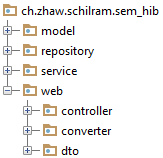
\includegraphics[width=0.2\columnwidth]{graphics/pakete.png}%
	\caption{Paketstruktur}
	\label{fig:Paketstruktur}
\end{figure}
\\
\textbf{model}\\
Im Paket \emph{model} sind die Model Klassen untergebracht welche von Hibernate für das OR Mapping genutzt werden. Sämtliche Model Klassen implementieren das Interface \emph{Uniquness}\\
\\
\textbf{repository}\\
Im Paket \emph{repository} sind sämtliche Sämtliche Interfaces welche das JPARepository Interface implementieren und für den Zugriff auf die Datenbank dienen.\\
\\
\textbf{service}\\
Das Paket \emph{service} beinhaltet für jede Model Klasse ein Service Interface und eine Service Klasse welche den Zugriff auf die Datenbank ermöglicht. Die Klasse \emph{AbstractCrudService} implementiert die CRUD Methoden welche durch die Interfaces \emph{CrudService} und \emph{ReadService} vorgegeben werden. Die Service Interfaces extenden jeweils das Interface \emph{CrudService} und werden von den Service Klassen welche auch den \emph{AbstractCrudService} extenden implementiert. Siehe dazu auch \autoref{fig:Klassendiagramm_service_repository}.  \\
\\
\textbf{web.controller}\\
Im Paket \emph{web.controller} sind die Controller Klassen abgelegt welche die Web Requests entgegennehmen und verarbeiten\\
\\
\textbf{web.converter}\\
Hier sind einerseits die Converter Klassen gespeichert, welche statische Methoden zur Umwandlung einer Model Klasse in die entsprechende DTO Klasse anbieten, sowie auch die Converter, welche gebraucht werden um über in Web Formularen als String übermittelte ID das zugehörige persistierte Objekts zu finden.\\
\\
\textbf{web.dto}\\
Im Pakte \emph{web.dto} sind die DTO bzw. Formular Klassen welche für die Formulareingabe genutzt werden abgelegt.

\subsection{Klassendiagramm}
Unten sind die Klassendiagramme der Pakete \emph{model} und \emph{service} aufgeführt.

\subsection{Klassendiagramm Paket model}

\begin{figure}[h]
\centering
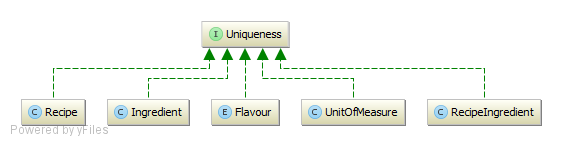
\includegraphics[width=0.6\columnwidth]{graphics/Klassendiagramm_model.png}%
	\caption{Klassendiagramm Paket \emph{model}}
	\label{fig:Klassendiagramm_model}
\end{figure}

\subsection{Klassendiagramm Pakete service und repository}
\begin{figure}[h]
\centering
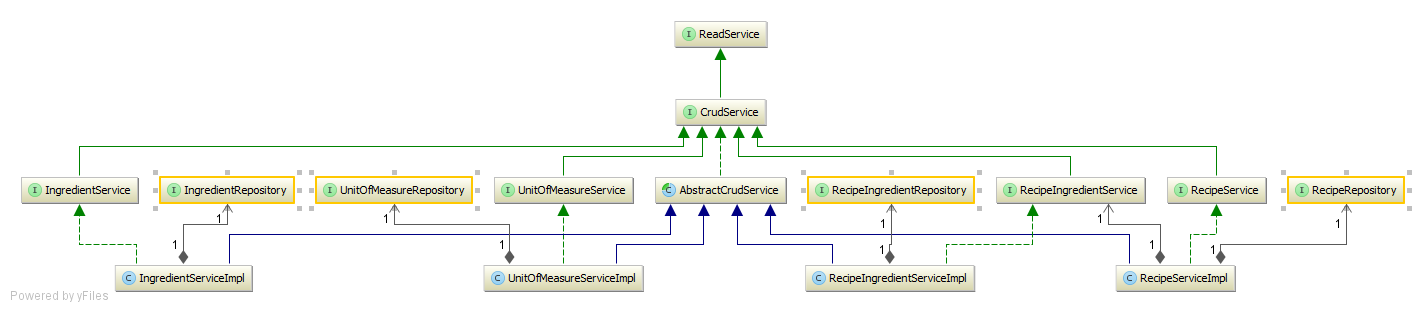
\includegraphics[width=1\columnwidth]{graphics/Klassendiagramm_service_repository.png}%
	\caption{Klassendiagramm Paket \emph{service}}
	\label{fig:Klassendiagramm_service_repository}
\end{figure}


\section{Konfigurationsfiles}\\
Im Ordner \emph{ressources} sind die Konfigurationsfiles hinterlegt.\\
\\
\textbf{application.properties}
In dieser Datei ist die Hibernate Konfiguration gespeichert. Um eine andere Datenbank oder einen anderen Datenbankuser zu verwenden müsste diese Datei angepasst werden.\\
\\
\textbf{root-context.xml}\\
Dies ist das Spring Basis Konfigurationsfile. Hier wird festgelegt in welchen Paketen Spring nach den Repository Klassen und Service Klassen sucht.\\
\\
\textbf{datasource-context.xml}\\
Hier wird Spring die Datenquelle bekanntgegeben. Die relevanten Daten werden aus dem Konfigurationsfile \emph{application.properties} ausgelesen.\\
\\
\textbf{dispatcher-context.xml}\\
Dies ist die Konfigurationsdatei für Spring MVC.\\
\\
\textbf{logback.xml}\\
Die Konfigurationsdatei für das Logging.



\section{Installation}

\subsection{Voraussetzungen}
Damit die Applikation läuft muss sie auf eine Datenbank zugreifen können. Zusätzlich wird Tomcat \cite{Tomcat} vorausgsetzt um die Web Applikation laufen zu lassen.

\subsection{Datenbank einrichten}
Die Applikation läuft mit PostgreSQL. PostgreSQL kann unter \url{http://www.postgresql.org/} heruntergeladen werden.

Nach der Installation von PostgreSQL muss der Benutzer angelegt werden. Standardmässig wird der Benutzer \emph{sem\_hib} mit dem Passwort \emph{sem\_hib} genutzt. Der Benutzer kann über das Gui oder mit folgendem SQL Statement erstellt werden.

\lstset{
	language=SQL,
	keywordstyle=\ttfamily,
	identifierstyle=\ttfamily,
	commentstyle=\color[rgb]{0.133,0.545,0.133},
	stringstyle=\ttfamily,
	showstringspaces=false,
	basicstyle=\small,
	tabsize=2,
	breaklines=true,
	prebreak = \raisebox{0ex}[0ex][0ex]{\ensuremath{\hookleftarrow}},
	breakatwhitespace=false,
	aboveskip={1.5\baselineskip},
  columns=fixed,
  upquote=true,
  extendedchars=true,
}
\begin{lstlisting}
CREATE ROLE sem_hib LOGIN
	ENCRYPTED PASSWORD 'md5198ad17e37731cbad30b3130a0a88919'
	VALID UNTIL 'infinity';
\end{lstlisting}

Nach der Erstellung des Benutzers muss noch die Datenbank erstellt werden. Der Datenbankbesitzer muss dabei auf den eben erstellten Benutzer festgelegt werden. Die Datenbank kann wahlweise über das Gui oder über das untenstehende SQL Statement erzeugt werden.

\begin{lstlisting}
CREATE DATABASE sem_hib
	WITH ENCODING='UTF8'
	OWNER=sem_hib
	CONNECTION LIMIT=-1;
\end{lstlisting}


\subsection{Tomcat einrichten}
Der Tomcat Server kann von \url{http://tomcat.apache.org/} heruntergeladen werden.
Nach der Installation von Tomcat kann die Applikation über das Management Interface installiert werden. Die Benötigte Datei heisst \emph{sem\_hib.war}. Alternativ kann dasFile \emph{sem\_hib.war} kann direkt in den Ordner \emph{webapps} von Tomcat kopiert werden.

\subsection{Applikation starten}
Nachdem die Applikation installiert ist kann über \ursl{http://localhost:8080/sem\_hib/} darauf zugegriffen werden.

\section{Applikation verwenden}
Die Applikation besteht aus den Teilen \emph{Zutaten}, \emph{Masseinheiten}, \emph{Rezepte} und \emph{Suche}.\\
Zuerst müssen Zutaten und Masseinheiten erfasst werden. Danach können diese beim Erfassen von Rezepten ausgewählt werden. Wenn einmal ein paar Rezepte erfasst sind, kann über die Suche nach Rezepten gesucht werden welche bestimmte Zutaten enthalten.

\subsection{Zutaten erfassen}
Einer Zutat kann ein Name gegeben werden und eine Beschreibung. Zusätzlich kann noch der Geschmack (Salzig, Süss, Sauer, Bitter oder Umami) agegeben werden.
\begin{figure}[h]
\centering
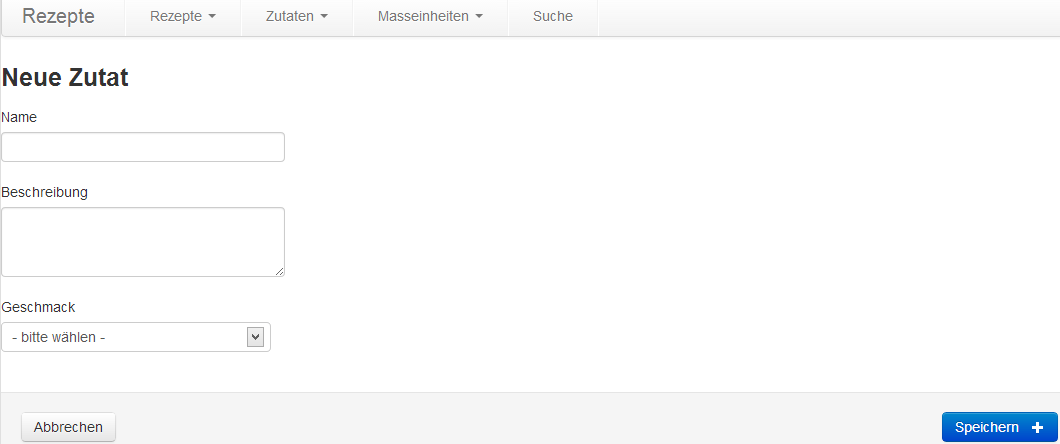
\includegraphics[width=0.5\columnwidth]{graphics/erfassen_zutat.png}%
	\caption{Zutat erfassen}
	\label{fig:erfassen_zutat}
\end{figure}

\subsection{Masseinheiten erfassen}
Der Masseinheit kann ein Key und ein Name gegeben werden. Ebenfalss kann noch eine Beschreibung hinzugefügt werden. Über den Key (z.B. EL für Esslöffel) wählt man beim Rezept dann die Masseinheit aus. 
\begin{figure}[h]
\centering
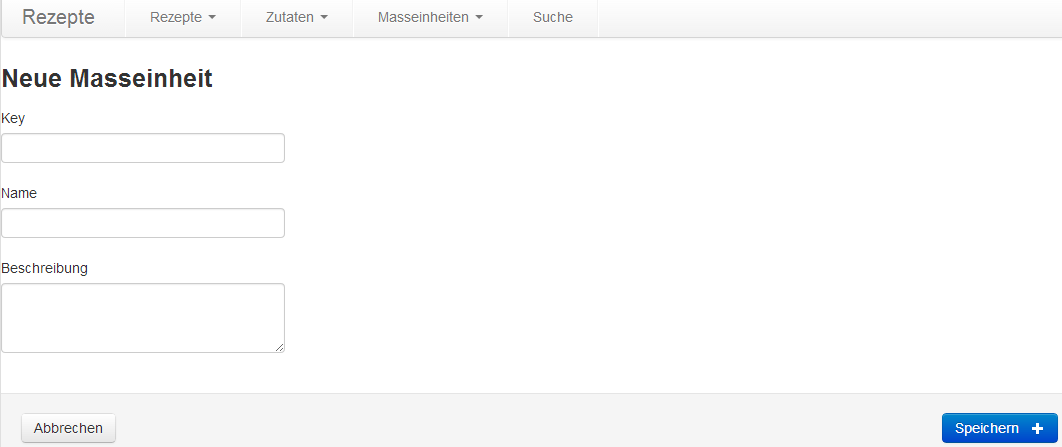
\includegraphics[width=0.5\columnwidth]{graphics/erfassen_masseinheit.png}%
	\caption{Masseinheit erfassen}
	\label{fig:erfassen_masseinheit}
\end{figure}

\subsection{Rezepte erfassen}
Beim Erfassen eines Rezeptes ist neben dem Namen natürlich wichtig, dass die Zutaten angegeben werden können. Über den Button \emph{Zeile hinzufügen} kann eine weitere Zutatenzeile hinzugefügt werden. Über das Löschen Icon neben der Zeile kann eine Zeile gelöscht werden. Im Feld \emph{Zubereitung} wird die Kochanleitung hinterlegt.
\begin{figure}[h]
\centering
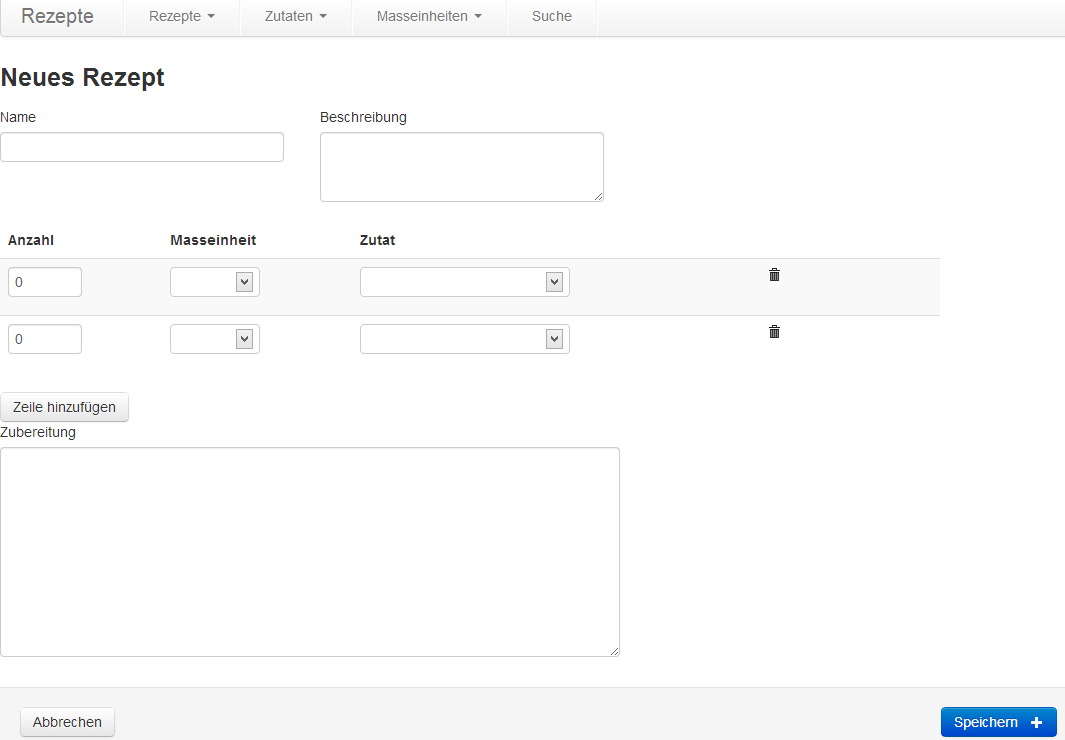
\includegraphics[width=0.5\columnwidth]{graphics/erfassen_rezept.png}%
	\caption{Rezept erfassen}
	\label{fig:erfassen_rezept}
\end{figure}

\subsection{Rezepte suchen}
Bei der Suche können bis zu drei Zutaten angegeben werden. Als Resultat werden alle Rezepte aufgelistet welche mindestens eine dieser Zutaten benötigen.
\chapter{Fazit}
\label{chap:Fazit}

Ich fand die Auseinandersetzung mit den genutzten Technologien spannend und sehr lehrreich. Ich bin überzeugt, dass ich die hier gewonnenen Erfahrungen weiter nutzen kann da ich in Zukunft noch öfters mit Hibernate arbeiten werde. Trotz, oder vielleicht auch wegen einiger nervenzehrender Momente hat mir die Arbeit auch viel Spass bereitet.

Bis ich die ersten Tests mit Hibernate erfolgreich hinter mich gebracht hatte dauerte es recht lange. Das war zwar einerseits frustrierend, zeigte mir aber auch wie wichtig das grundlegende Verständnis für die genutzten Technologien ist. Einige im Internet verfügbare Tutorials gehen total verschiedene Wege und zeigen zum Teil nur einen kleinen Ausschnitt. Daraus jeweils die für das eigene Problem wichtigen Teile herauszufiltern ist manchmal ziemlich knifflig. Dies ist vor allem der Fall wenn man sich mit mehreren Frameworks gleichzeitig auseinandersetzt welche man noch nicht kennt.

Ich habe auch den reinen Programmieraufwand unterschätzt, da ich mich manchmal mit Fehlern aufgehalten habe, welche ich bestimmt nicht nochmals machen werde. Ein Beispiel hierfür ist, dass beim Editieren eines Rezeptes nicht die richtigen Masseinheiten und Zutaten angezeigt wurden obwohl ich mit dem Debugger sehen konnte, dass die richtigen Eigenschauften ausgelesen wurden und auch im DTO die Angaben stimmten. Da ich in der Model Klasse aber die \emph{equals\(\)} Methode nicht überschrieben hatte, konnten die Objekte nicht verglichen werden.

Ich hätte die Applikation gerne noch ausgebaut und verfeinert. Leider bin ich nicht mehr dazu gekommen eine Validierung zu implementieren. Dies wäre sicher einer der nächsten Schritte. Ein weiterer Punkt welchem ich gerne Beachtung geschenkt hätte wäre die internationalisierung gewesen.

\listoffigures
\nocite{*} 
\bibliography{bib/bib1}{}
\bibliographystyle{plain}
%\bibliographystyle{alphadin}
%\bibliographystyle{plain}
\end{spacing}
\end{document}